\documentclass{ximera}  


%\usepackage{todonotes}
%\usepackage{mathtools} %% Required for wide table Curl and Greens
%\usepackage{cuted} %% Required for wide table Curl and Greens
\newcommand{\todo}{}

\usepackage{esint} % for \oiint
\ifxake%%https://math.meta.stackexchange.com/questions/9973/how-do-you-render-a-closed-surface-double-integral
\renewcommand{\oiint}{{\large\bigcirc}\kern-1.56em\iint}
\fi


\graphicspath{
  {./}
  {jpg}
  {ximeraTutorial/}
  {basicPhilosophy/}
  {functionsOfSeveralVariables/}
  {normalVectors/}
  {lagrangeMultipliers/}
  {vectorFields/}
  {greensTheorem/}
  {shapeOfThingsToCome/}
  {dotProducts/}
  {partialDerivativesAndTheGradientVector/}
  {../productAndQuotientRules/exercises/}
  {../motionAndPathsInSpace/exercises/}
  {../normalVectors/exercisesParametricPlots/}
  {../continuityOfFunctionsOfSeveralVariables/exercises/}
  {../partialDerivativesAndTheGradientVector/exercises/}
  {../directionalDerivativeAndChainRule/exercises/}
  {../commonCoordinates/exercisesCylindricalCoordinates/}
  {../commonCoordinates/exercisesSphericalCoordinates/}
  {../greensTheorem/exercisesCurlAndLineIntegrals/}
  {../greensTheorem/exercisesDivergenceAndLineIntegrals/}
  {../shapeOfThingsToCome/exercisesDivergenceTheorem/}
  {../greensTheorem/}
  {../shapeOfThingsToCome/}
  {../separableDifferentialEquations/exercises/}
  {vectorFields/}
}

\newcommand{\mooculus}{\textsf{\textbf{MOOC}\textnormal{\textsf{ULUS}}}}

\usepackage{tkz-euclide}\usepackage{tikz}
\usepackage{tikz-cd}
\usetikzlibrary{arrows}
\tikzset{>=stealth,commutative diagrams/.cd,
  arrow style=tikz,diagrams={>=stealth}} %% cool arrow head
\tikzset{shorten <>/.style={ shorten >=#1, shorten <=#1 } } %% allows shorter vectors

\usetikzlibrary{backgrounds} %% for boxes around graphs
\usetikzlibrary{shapes,positioning}  %% Clouds and stars
\usetikzlibrary{matrix} %% for matrix
\usepgfplotslibrary{polar} %% for polar plots
\usepgfplotslibrary{fillbetween} %% to shade area between curves in TikZ
\usetkzobj{all}
\usepackage[makeroom]{cancel} %% for strike outs
%\usepackage{mathtools} %% for pretty underbrace % Breaks Ximera
%\usepackage{multicol}
\usepackage{pgffor} %% required for integral for loops



%% http://tex.stackexchange.com/questions/66490/drawing-a-tikz-arc-specifying-the-center
%% Draws beach ball
\tikzset{pics/carc/.style args={#1:#2:#3}{code={\draw[pic actions] (#1:#3) arc(#1:#2:#3);}}}



\usepackage{array}
\setlength{\extrarowheight}{+.1cm}
\newdimen\digitwidth
\settowidth\digitwidth{9}
\def\divrule#1#2{
\noalign{\moveright#1\digitwidth
\vbox{\hrule width#2\digitwidth}}}





\newcommand{\RR}{\mathbb R}
\newcommand{\R}{\mathbb R}
\newcommand{\N}{\mathbb N}
\newcommand{\Z}{\mathbb Z}

\newcommand{\sagemath}{\textsf{SageMath}}


%\renewcommand{\d}{\,d\!}
\renewcommand{\d}{\mathop{}\!d}
\newcommand{\dd}[2][]{\frac{\d #1}{\d #2}}
\newcommand{\pp}[2][]{\frac{\partial #1}{\partial #2}}
\renewcommand{\l}{\ell}
\newcommand{\ddx}{\frac{d}{\d x}}

\newcommand{\zeroOverZero}{\ensuremath{\boldsymbol{\tfrac{0}{0}}}}
\newcommand{\inftyOverInfty}{\ensuremath{\boldsymbol{\tfrac{\infty}{\infty}}}}
\newcommand{\zeroOverInfty}{\ensuremath{\boldsymbol{\tfrac{0}{\infty}}}}
\newcommand{\zeroTimesInfty}{\ensuremath{\small\boldsymbol{0\cdot \infty}}}
\newcommand{\inftyMinusInfty}{\ensuremath{\small\boldsymbol{\infty - \infty}}}
\newcommand{\oneToInfty}{\ensuremath{\boldsymbol{1^\infty}}}
\newcommand{\zeroToZero}{\ensuremath{\boldsymbol{0^0}}}
\newcommand{\inftyToZero}{\ensuremath{\boldsymbol{\infty^0}}}



\newcommand{\numOverZero}{\ensuremath{\boldsymbol{\tfrac{\#}{0}}}}
\newcommand{\dfn}{\textbf}
%\newcommand{\unit}{\,\mathrm}
\newcommand{\unit}{\mathop{}\!\mathrm}
\newcommand{\eval}[1]{\bigg[ #1 \bigg]}
\newcommand{\seq}[1]{\left( #1 \right)}
\renewcommand{\epsilon}{\varepsilon}
\renewcommand{\phi}{\varphi}


\renewcommand{\iff}{\Leftrightarrow}

\DeclareMathOperator{\arccot}{arccot}
\DeclareMathOperator{\arcsec}{arcsec}
\DeclareMathOperator{\arccsc}{arccsc}
\DeclareMathOperator{\si}{Si}
\DeclareMathOperator{\scal}{scal}
\DeclareMathOperator{\sign}{sign}


%% \newcommand{\tightoverset}[2]{% for arrow vec
%%   \mathop{#2}\limits^{\vbox to -.5ex{\kern-0.75ex\hbox{$#1$}\vss}}}
\newcommand{\arrowvec}[1]{{\overset{\rightharpoonup}{#1}}}
%\renewcommand{\vec}[1]{\arrowvec{\mathbf{#1}}}
\renewcommand{\vec}[1]{{\overset{\boldsymbol{\rightharpoonup}}{\mathbf{#1}}}\hspace{0in}}

\newcommand{\point}[1]{\left(#1\right)} %this allows \vector{ to be changed to \vector{ with a quick find and replace
\newcommand{\pt}[1]{\mathbf{#1}} %this allows \vec{ to be changed to \vec{ with a quick find and replace
\newcommand{\Lim}[2]{\lim_{\point{#1} \to \point{#2}}} %Bart, I changed this to point since I want to use it.  It runs through both of the exercise and exerciseE files in limits section, which is why it was in each document to start with.

\DeclareMathOperator{\proj}{\mathbf{proj}}
\newcommand{\veci}{{\boldsymbol{\hat{\imath}}}}
\newcommand{\vecj}{{\boldsymbol{\hat{\jmath}}}}
\newcommand{\veck}{{\boldsymbol{\hat{k}}}}
\newcommand{\vecl}{\vec{\boldsymbol{\l}}}
\newcommand{\uvec}[1]{\mathbf{\hat{#1}}}
\newcommand{\utan}{\mathbf{\hat{t}}}
\newcommand{\unormal}{\mathbf{\hat{n}}}
\newcommand{\ubinormal}{\mathbf{\hat{b}}}

\newcommand{\dotp}{\bullet}
\newcommand{\cross}{\boldsymbol\times}
\newcommand{\grad}{\boldsymbol\nabla}
\newcommand{\divergence}{\grad\dotp}
\newcommand{\curl}{\grad\cross}
%\DeclareMathOperator{\divergence}{divergence}
%\DeclareMathOperator{\curl}[1]{\grad\cross #1}
\newcommand{\lto}{\mathop{\longrightarrow\,}\limits}

\renewcommand{\bar}{\overline}

\colorlet{textColor}{black}
\colorlet{background}{white}
\colorlet{penColor}{blue!50!black} % Color of a curve in a plot
\colorlet{penColor2}{red!50!black}% Color of a curve in a plot
\colorlet{penColor3}{red!50!blue} % Color of a curve in a plot
\colorlet{penColor4}{green!50!black} % Color of a curve in a plot
\colorlet{penColor5}{orange!80!black} % Color of a curve in a plot
\colorlet{penColor6}{yellow!70!black} % Color of a curve in a plot
\colorlet{fill1}{penColor!20} % Color of fill in a plot
\colorlet{fill2}{penColor2!20} % Color of fill in a plot
\colorlet{fillp}{fill1} % Color of positive area
\colorlet{filln}{penColor2!20} % Color of negative area
\colorlet{fill3}{penColor3!20} % Fill
\colorlet{fill4}{penColor4!20} % Fill
\colorlet{fill5}{penColor5!20} % Fill
\colorlet{gridColor}{gray!50} % Color of grid in a plot

\newcommand{\surfaceColor}{violet}
\newcommand{\surfaceColorTwo}{redyellow}
\newcommand{\sliceColor}{greenyellow}




\pgfmathdeclarefunction{gauss}{2}{% gives gaussian
  \pgfmathparse{1/(#2*sqrt(2*pi))*exp(-((x-#1)^2)/(2*#2^2))}%
}


%%%%%%%%%%%%%
%% Vectors
%%%%%%%%%%%%%

%% Simple horiz vectors
\renewcommand{\vector}[1]{\left\langle #1\right\rangle}


%% %% Complex Horiz Vectors with angle brackets
%% \makeatletter
%% \renewcommand{\vector}[2][ , ]{\left\langle%
%%   \def\nextitem{\def\nextitem{#1}}%
%%   \@for \el:=#2\do{\nextitem\el}\right\rangle%
%% }
%% \makeatother

%% %% Vertical Vectors
%% \def\vector#1{\begin{bmatrix}\vecListA#1,,\end{bmatrix}}
%% \def\vecListA#1,{\if,#1,\else #1\cr \expandafter \vecListA \fi}

%%%%%%%%%%%%%
%% End of vectors
%%%%%%%%%%%%%

%\newcommand{\fullwidth}{}
%\newcommand{\normalwidth}{}



%% makes a snazzy t-chart for evaluating functions
%\newenvironment{tchart}{\rowcolors{2}{}{background!90!textColor}\array}{\endarray}

%%This is to help with formatting on future title pages.
\newenvironment{sectionOutcomes}{}{}



%% Flowchart stuff
%\tikzstyle{startstop} = [rectangle, rounded corners, minimum width=3cm, minimum height=1cm,text centered, draw=black]
%\tikzstyle{question} = [rectangle, minimum width=3cm, minimum height=1cm, text centered, draw=black]
%\tikzstyle{decision} = [trapezium, trapezium left angle=70, trapezium right angle=110, minimum width=3cm, minimum height=1cm, text centered, draw=black]
%\tikzstyle{question} = [rectangle, rounded corners, minimum width=3cm, minimum height=1cm,text centered, draw=black]
%\tikzstyle{process} = [rectangle, minimum width=3cm, minimum height=1cm, text centered, draw=black]
%\tikzstyle{decision} = [trapezium, trapezium left angle=70, trapezium right angle=110, minimum width=3cm, minimum height=1cm, text centered, draw=black]




 
\title{Example of circuit analysis with phasors} 
\author{Milica Markovic} 
\outcome{Apply phasor transformation to a time-domain equation to obtain frequency-domain equation.}
\begin{document}  
\begin{abstract}  
Phasors are essential tool in circuit analysis.
\end{abstract}  
\maketitle    




 Step-by-step instructions on how to solve circuits using phasors:
\begin{enumerate}
\item adopt cosine reference for generator voltage or current. 
\item replace all impedances with their phasor expressions,
\item write KVL and KCL or use other Network Analysis techniques.
\item find the phasor expression for the required current or voltage. 
\item calculate phasors 
\item sketch the phasor diagram
\item multiply the phasor with $e^{j \omega t}$  
\item find the real part of the above expression to get the current in the time domain.
\end{enumerate}


It is customary in Electrical Engineering to use  $\cos( \omega t)$ for our time-domain signal, and we call these phasors "cosine reference phasors."  If the generator in a circuit is  $\sin (\omega t)$, we first have to convert the sin function to a cosine. To do that, subtract $90^o$ from the phase of the sinusoid, because $\sin( \omega t) = \cos(\omega t - 90^o)$.

\begin{example}
Using Vectors to Represent Phasors in an example

A series RC circuit shown in Figure \ref{RCcircADS}. The circuit is driven with a frequency of 1\,GHz $v_s(t)=  \cos \omega t$, and R=1k$\Omega $, C= ${\frac{1}{2\pi }10}^{-12}$F. 
 


\begin{enumerate}
\item  Identify magnitude, phase, and time-delay of the source voltage.

\item  Calculate magnitude, phase, and time-delay of the voltage across the resistor.

\item  Calculate magnitude, phase, and time-delay of the voltage across the capacitor.

\item  The simulated voltage magnitude across the resistor is about 0.5V, and the simulated voltage across the capacitor is about 0.85V.  If we use KVL $ 0.85V+0.5V \neq 1V$. Why? Look at Figure \ref{f112}  to answer this question.

\item Sketch the phasor diagram of voltages in the circuit. 

\end{enumerate}

\begin{explanation} 
The magnitude of the voltage source is 1; the phase and time-delays are zero. To find the voltages and currents in the circuit, we will follow the process outlined above.

Solving for voltages and currents in the circuit.
 \begin{enumerate}
\item The generator is already given in terms of the cosine function. The phasor of this voltage is $\tilde{V}_s= 1$ 
\item replace all impedances with their phasor expressions. R is not changed, and the impedance of a capacitor is $Z_c=\frac{1}{j \omega C}$.
\item  Use Kirchoff's Voltage law 

\begin{eqnarray}
\tilde{V}_s  = R \tilde{I}    + \frac{\tilde{I}}{j \omega C}  
\end{eqnarray}

\item find the phasor expression for the required current or voltage. 

\begin{eqnarray}
\tilde{I}  = \frac{\tilde{V}_s}{ R    + \frac{1}{j \omega C} } \\
\tilde{V}_R = R \tilde{I} = R \frac{\tilde{V}_s}{ R    + \frac{1}{j \omega C} }  \\
\tilde{V}_C = Z_c \tilde{I} =  \frac{1}{ j \omega C} \frac{\tilde{V}_s}{ R    + \frac{1}{j \omega C} }  
\end{eqnarray}

\item calculate the currents and voltages from the above expressions

\begin{eqnarray}
\tilde{I}  = 0.54 e^{j 58^o} \unit{mA} \\
\tilde{V_R} = 0.54  e^{j 58^o} \unit{V}\\
\tilde{V_C} =   0.85 e^{-j 32^o}  \unit{V}
\end{eqnarray}

\item When you calculate the magnitudes and phases of the voltages in the RC circuit, draw three complex numbers to represent all three vectors' magnitude and phases, as in Figure \ref{PP}. The three points denote the three position-vectors, as shown in Figure \ref{f112}. We must use vector addition to add the voltages on the resistor and capacitor to obtain the generator's voltage. The magnitudes of voltages do not add simply as real numbers, because the voltages have different phases. Complex numbers magnitudes are added only if their phases are the same; in other words, if the phasors point in the same direction, as is the case for purely resistive circuits. However, if we use vector addition (or complex number addition) in any circuit, we will get that the vectors of voltages add up to the source voltage.
\item multiply the phasor with $e^{j \omega t}$  

\begin{eqnarray}
0.54 e^{j 58^o} e^{j \omega t} = 0.54 e^{j(\omega t + 58^o)}\\
0.54  e^{j 58^o} e^{j \omega t} =0.54  e^{j( \omega t + 58^o)}\\
 0.85 e^{-j 32^o}e^{j \omega t} =0.85 e^{j(\omega t - 32^o)}
\end{eqnarray}
\item find the real part of the above expression to get the current in the time domain. Time domain signals are shown in Figure \ref{SSangle}.

\begin{eqnarray}
i(t)= \Re \{  0.54 e^{j(\omega t + 58^o)}  \} =0.54 \cos(\omega t + 58^o)  \unit{mA}  \\
v_R(t)= \Re \{ 0.54  e^{j( \omega t + 58^o)} \} = 0.54 \cos(\omega t + 58^o) \unit{V}   \\ 
v_C(t) =\Re \{ 0.85 e^{j(\omega t - 32^o)}    \} = 0.85 \cos(\omega t - 32^o) \unit{V}
\end{eqnarray}
\end{enumerate}
 
 To find time-delay for each signal, we will use the equation $T=\frac{\Theta}{2 \pi f}$.  Since angles above are in degrees, we need to convert degrees to radians. $\frac{\Theta_{deg}*2 \pi /360}{2 \pi f}=\frac{ \Theta_{deg}}{360 f}  $. Time-delays are as follows:
 
 \begin{eqnarray}
 \tau_i= 160 \unit{ns} \\
 \tau_Vr= 160 \unit{ns} \\
 \tau_Vc=- 88 \unit{ns}  
 \end{eqnarray}
 
 
 


\begin{figure}[htbp]
%\vspace*{-0.5cm}
\begin{center}
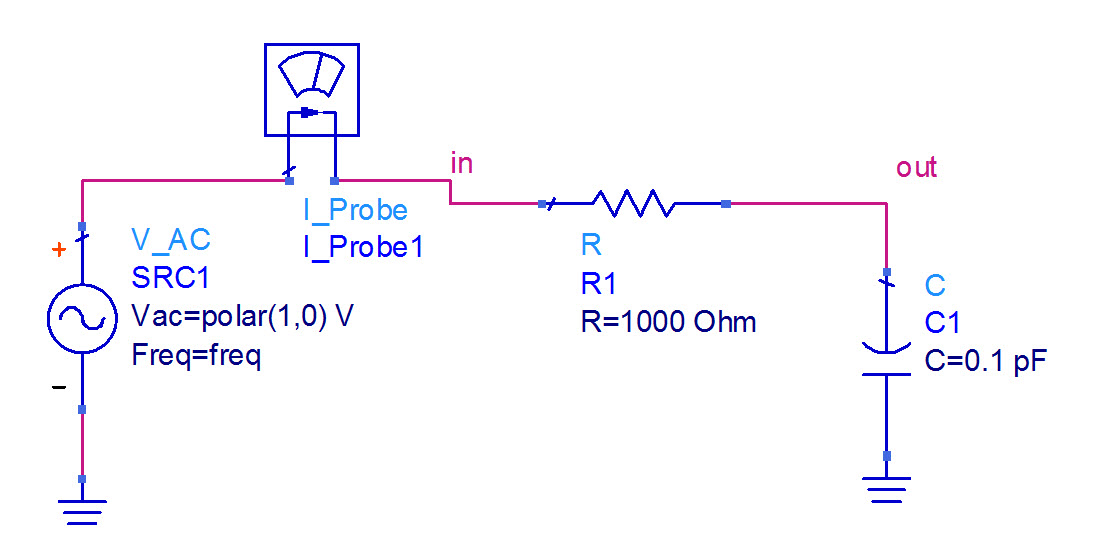
\includegraphics[scale=0.2]{../jpg/RCcircADS.jpg}
\end{center}
\caption{\label{RCcircADS} RC circuit in ADS.}
\end{figure}


\begin{figure}[htbp]
%\vspace*{-0.5cm}
\begin{center}
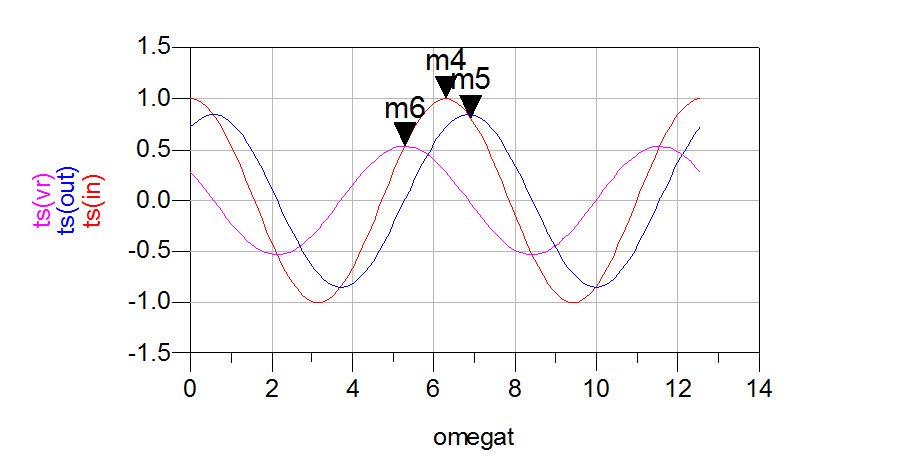
\includegraphics[scale=0.3]{../jpg/voltagesinRCcircRadADS}
\end{center}
\caption{\label{SSangle} Sinusoidal signal as a function of angle $\omega t$}
\end{figure}


\begin{figure}[htbp]
%\vspace*{-0.5cm}
\begin{center}
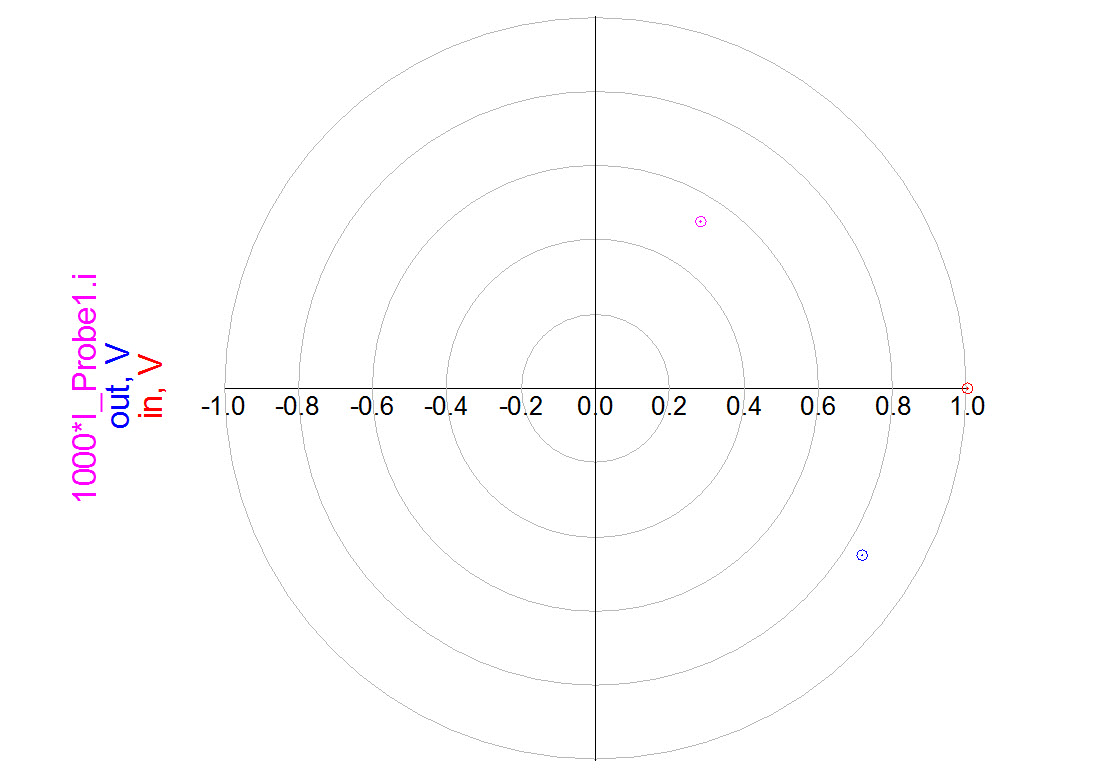
\includegraphics[scale=0.2]{../jpg/RCvoltPolarPlotADS.jpg}
\end{center}
\caption{\label{PP} Points represent polar plot of complex voltages in RC circuit.}
\end{figure}


\begin{figure}[htbp]
%\vspace*{-0.5cm}
\begin{center}
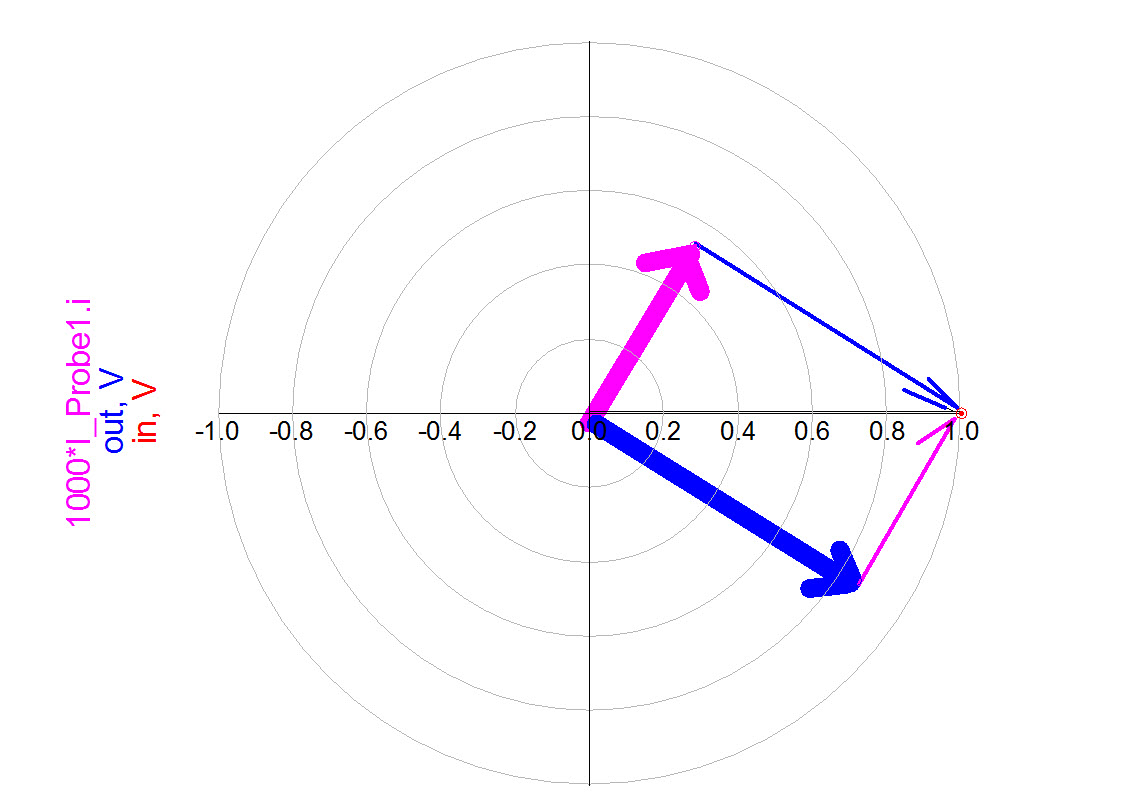
\includegraphics[scale=0.2]{../jpg/RCvoltPolarPlotVectors.jpg}
\end{center}
\caption{\label{f112} Vectors are drawn in the polar plot of complex voltages in RC circuit. Note how they add up to 1V with vector addition.}
\end{figure}





\end{explanation}



\end{example}

\newpage


\begin{example}
Observe the vector phasor diagram for an RC and an RL circuit below. How are the vector diagrams the same, and how are they different when the circuit's parameters change?
\subsection{Series RC Circuit}
\begin{center}  
\geogebra{h4bxa4rk}{900}{600}  
\end{center} 

\subsection{Series RL Circuit}
\begin{center}  
\geogebra{xuq8wchs}{900}{600}  
\end{center}
\end{example}
\end{document} 
